\shorthandoff{"}
\chapter{Diskussion}
\label{ch:diskussion}
Allgemeine Datenanalyse\\
- Teilnehmende Mitarbeiter N=23\\

Fähigkeiten im Intranet\\
Es wurden insgesamt 643 Bewertungen für Fähigkeiten im Intranet vergeben. Das entspricht ca. 30 vergebenen Bewertungen pro Person. Diese Bewertungen verteilen sich auf insgesamt 212 unterschiedliche Fähigkeiten.

Long Tail: 9 Fähigkeiten haben 10 oder mehr Bewertungen --> Entspricht ca. 4,25 Prozent; 151 Fähigkeiten haben 3 oder weniger Bewertungen --> Entspricht ca. 71,23 Prozent. Meisten Bewertungen erhielt Java mit 16 Bewertungen, dicht gefolgt von Spring Boot mit 15 Bewertungen. Long Tail auch bei grafischer Darstellung der Fähigkeiten zu erkennen:

\begin{figure}[h]
	\centering
	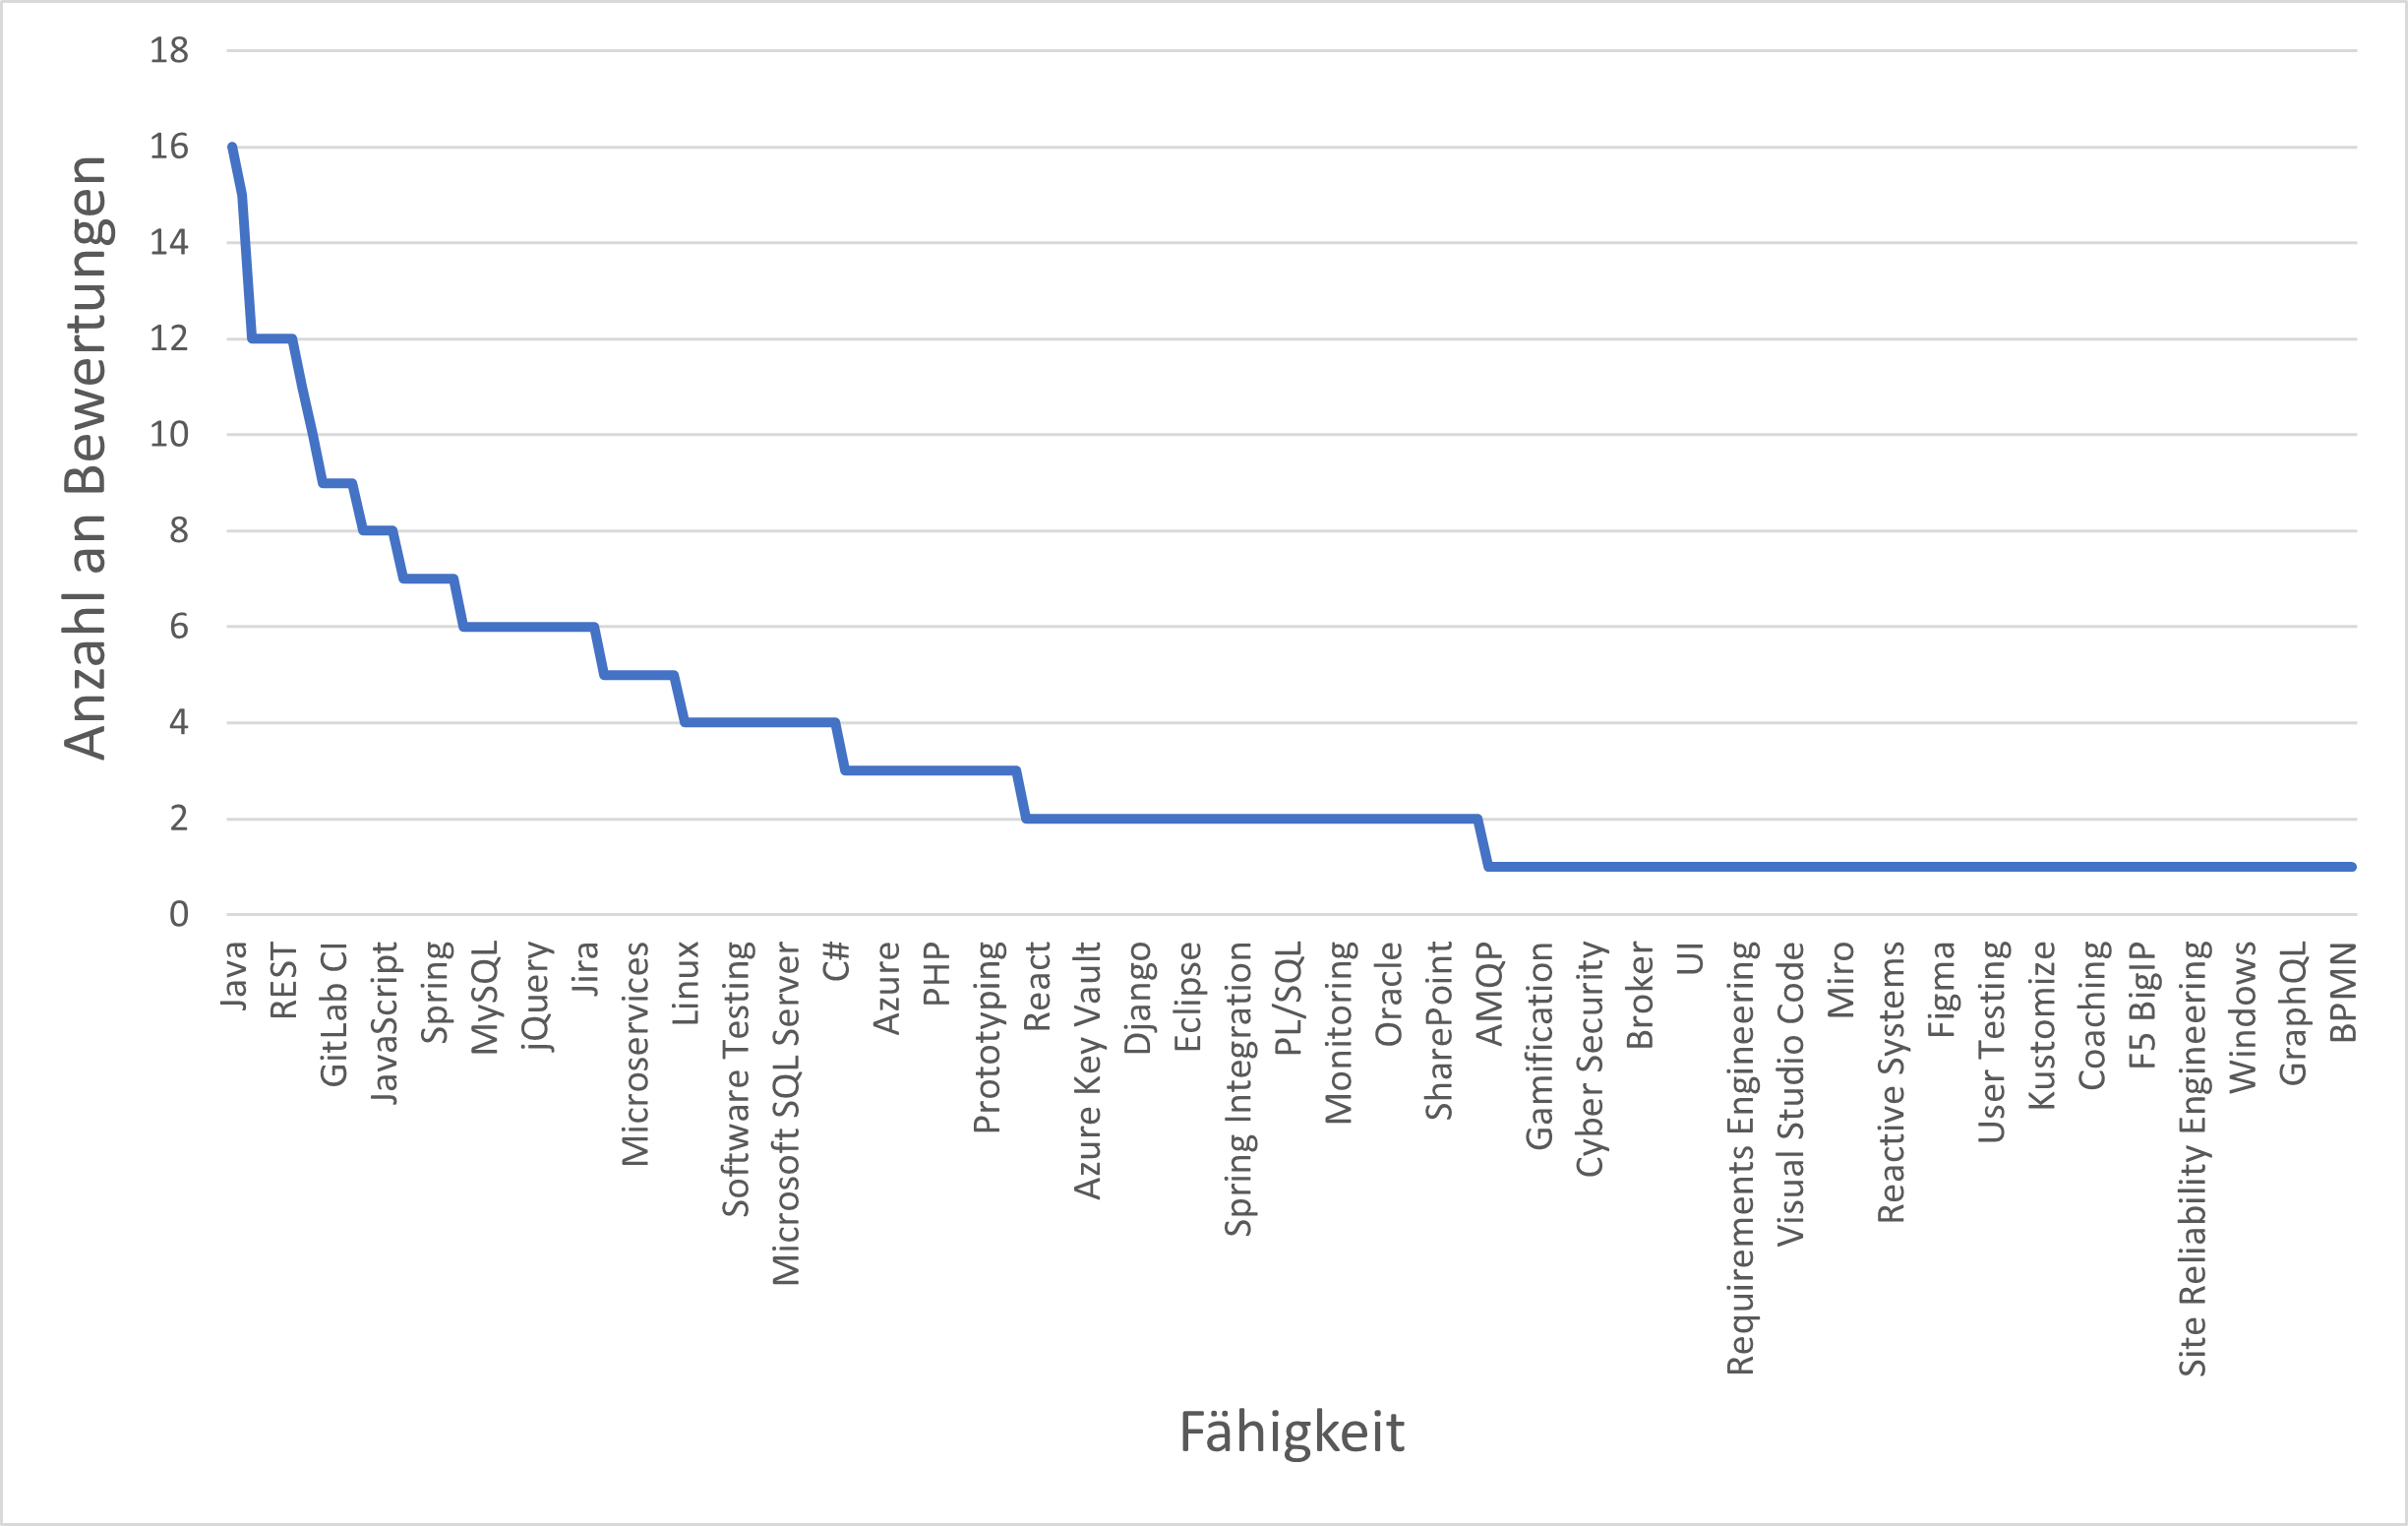
\includegraphics[width=1\textwidth]{gfx/long-tail-intranet.png}
	\caption{Langer (Ratten-)Schwanz bei Fähigkeitsbewertungen im EXXETA-Intranet}
	\label{fig:diskussion:abb1}
\end{figure}

Kaltstart: 4 Nutzer (17,39 Prozent) haben gar keine Fähigkeiten angegeben / Es sind immer mind. 19 andere Personen auf einem Skill verbunden

\newpage
- Link aufs Intranetprofil

\shorthandon{"}
